\documentclass[10pt,a4paper]{article}
\usepackage[top=1.0cm, bottom=1.0cm, left=1.5cm, right=1.5cm]{geometry}
\usepackage{tikz}
\usepackage{xcolor}
\usepackage{enumitem}
\usepackage[T1]{fontenc}
\usetikzlibrary{arrows.meta, shapes.geometric, positioning}
\pagestyle{empty}

\definecolor{cyellow}{RGB}{255,220,100}
\definecolor{cblue}{RGB}{100,180,255}
\definecolor{cgreen}{RGB}{100,210,140}
\definecolor{cpurple}{RGB}{200,150,255}
\definecolor{cred}{RGB}{255,140,140}
\definecolor{cgray}{RGB}{240,240,240}

\begin{document}

\begin{center}
{\large\textbf{COLDSTART --- System Architecture}}\\[3pt]
{\small
Abhishek Doke (\texttt{abhishekdoke233@gmail.com}) \quad
Nikhil Dhamdhere (\texttt{dhamdherenikhil75@gmail.com})\\[1pt]
Joanna Dharwadkar (\texttt{dharwadkarjoanna@gmail.com}) \quad
Geetanjali Bejjalwar (\texttt{bejjalwargeetanjali@gmail.com})
}\\[2pt]
{\small\textit{Guide: Dr.\ Alpana Adsul} \quad
Dept.\ of Computer Engineering,
Dr.\ D.Y.\ Patil College of Engineering \& Innovation, Varale, Talegaon, Pune \quad 2024--25}
\end{center}
\noindent\rule{\linewidth}{0.8pt}
\vspace{0.1cm}

\begin{center}
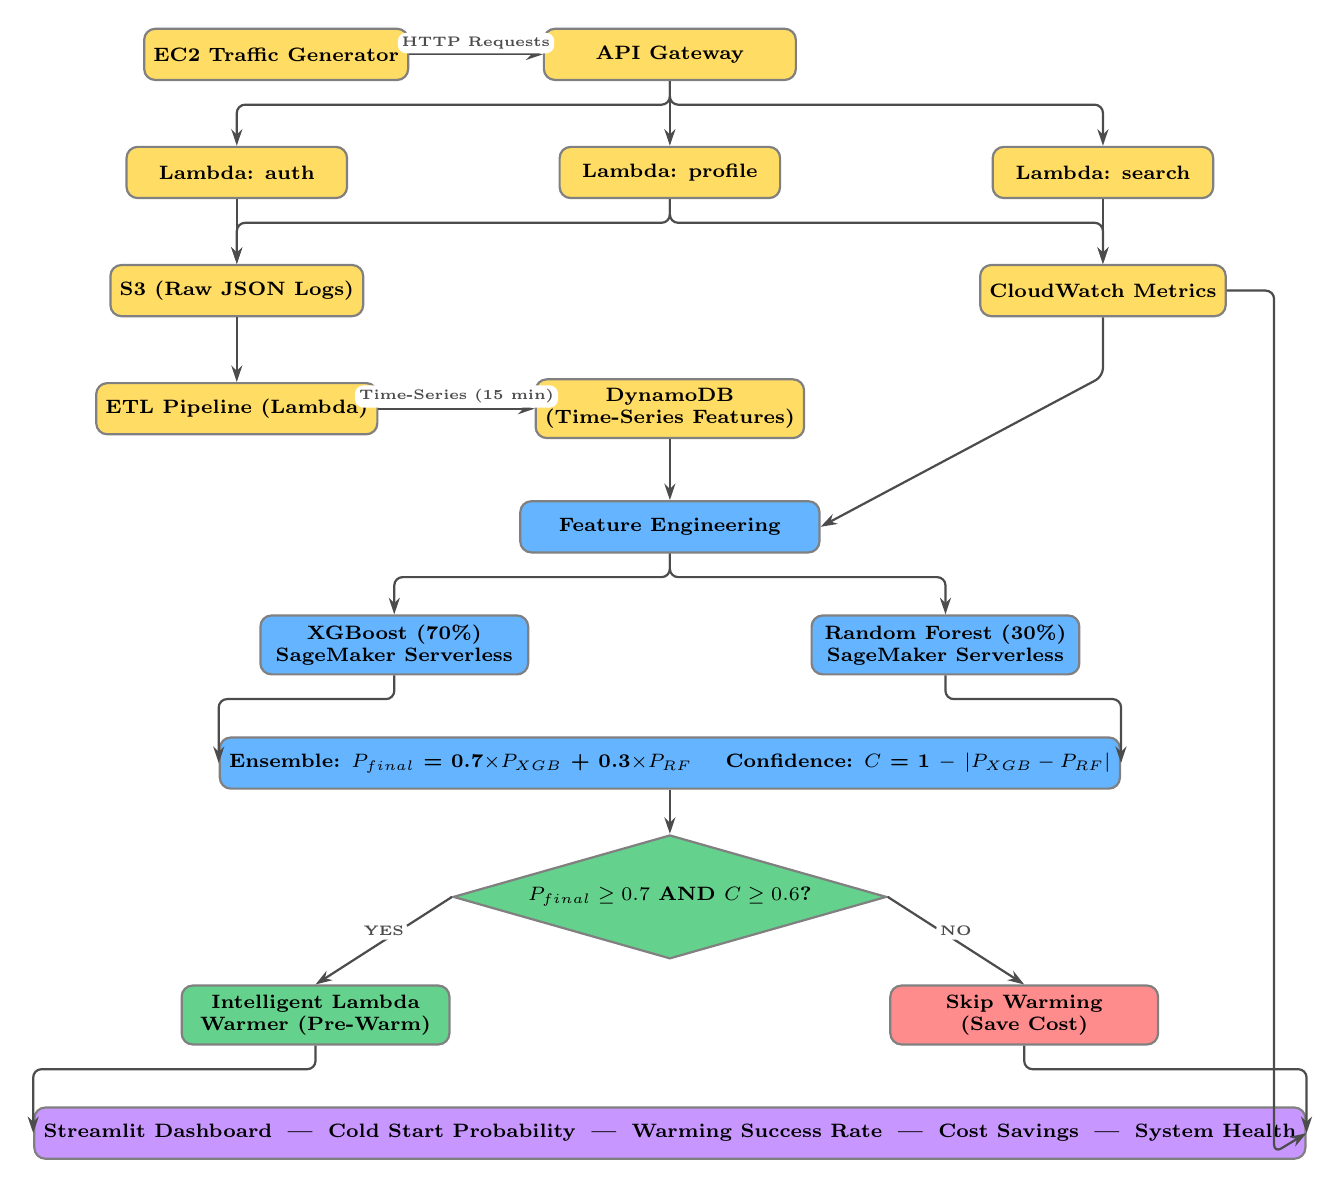
\begin{tikzpicture}[
  % Professional arrow style
  arr/.style={
    -{Stealth[length=6pt, width=4pt]},
    line width=0.8pt,
    color=black!70,
    rounded corners=3pt
  },
  % Box style
  box/.style={
    rectangle, rounded corners=4pt,
    draw=black!50, line width=0.8pt,
    minimum height=0.65cm,
    align=center, font=\scriptsize\bfseries
  },
  % Label on arrow
  albl/.style={font=\tiny\bfseries, fill=white, inner sep=1.5pt,
               text=black!70}
]

%% ─────────────────────────────────────────────────────────────────────────────
%% All nodes placed with absolute (x,y) coordinates
%% y increases downward (standard TikZ with positive y = up, so we use negative)
%% ─────────────────────────────────────────────────────────────────────────────

%% ROW 1  ── Traffic Generation ────────────────────────────────────────────────
\node[box, fill=cyellow, minimum width=3.2cm] (ec2)   at (2.5, 0)   {EC2 Traffic Generator};
\node[box, fill=cyellow, minimum width=3.2cm] (apigw) at (7.5, 0)   {API Gateway};

%% ROW 2  ── Lambda Functions ──────────────────────────────────────────────────
\node[box, fill=cyellow, minimum width=2.8cm] (la) at (2.0, -1.5)  {Lambda: auth};
\node[box, fill=cyellow, minimum width=2.8cm] (lp) at (7.5, -1.5)  {Lambda: profile};
\node[box, fill=cyellow, minimum width=2.8cm] (ls) at (13.0,-1.5)  {Lambda: search};

%% ROW 3  ── Storage ───────────────────────────────────────────────────────────
\node[box, fill=cyellow, minimum width=3.0cm] (s3raw) at (2.0, -3.0)
  {S3 (Raw JSON Logs)};
\node[box, fill=cyellow, minimum width=3.0cm] (cw)  at (13.0,-3.0)  {CloudWatch Metrics};

%% ROW 4  ── ETL ───────────────────────────────────────────────────────────────
\node[box, fill=cyellow, minimum width=3.0cm] (etl) at (2.0, -4.5)
  {ETL Pipeline (Lambda)};
\node[box, fill=cyellow, minimum width=3.0cm] (dyn)  at (7.5, -4.5)
  {DynamoDB\\(Time-Series Features)};

%% ROW 5  ── Feature Engineering ──────────────────────────────────────────────
\node[box, fill=cblue, minimum width=3.8cm]   (fe)  at (7.5, -6.0)  {Feature Engineering};

%% ROW 6  ── ML Models ────────────────────────────────────────────────────────
\node[box, fill=cblue, minimum width=3.4cm]   (xgb) at (4.0, -7.5)
  {XGBoost (70\%)\\SageMaker Serverless};
\node[box, fill=cblue, minimum width=3.4cm]   (rf)  at (11.0,-7.5)
  {Random Forest (30\%)\\SageMaker Serverless};

%% ROW 7  ── Ensemble ─────────────────────────────────────────────────────────
\node[box, fill=cblue, minimum width=8.5cm]   (ens) at (7.5, -9.0)
  {Ensemble: $P_{final}$ = 0.7$\times P_{XGB}$ + 0.3$\times P_{RF}$
   \quad Confidence: $C$ = 1 $-$ $|P_{XGB} - P_{RF}|$};

%% ROW 8  ── CBW Decision ─────────────────────────────────────────────────────
\node[diamond, fill=cgreen, draw=black!50, line width=0.8pt,
      minimum width=5.5cm, minimum height=1.0cm,
      align=center, font=\scriptsize\bfseries, aspect=3.5]
  (cbw) at (7.5,-10.7)
  {$P_{final} \geq 0.7$ \textbf{AND} $C \geq 0.6$?};

%% ROW 9  ── Actions ──────────────────────────────────────────────────────────
\node[box, fill=cgreen, minimum width=3.4cm]  (iw)   at (3.0,-12.2)
  {Intelligent Lambda\\Warmer (Pre-Warm)};
\node[box, fill=cred,   minimum width=3.4cm]  (skip) at (12.0,-12.2)
  {Skip Warming\\(Save Cost)};

%% ROW 10 ── Dashboard ────────────────────────────────────────────────────────
\node[box, fill=cpurple, minimum width=14.5cm] (dash) at (7.5,-13.7)
  {Streamlit Dashboard \;|\; Cold Start Probability \;|\;
   Warming Success Rate \;|\; Cost Savings \;|\; System Health};

%% ─────────────────────────────────────────────────────────────────────────────
%% ARROWS  ── all orthogonal, no crossings
%% ─────────────────────────────────────────────────────────────────────────────

%% EC2 → API Gateway (horizontal)
\draw[arr] (ec2.east) -- node[albl,above]{HTTP Requests} (apigw.west);

%% API Gateway → Lambda auth (down-left)
\draw[arr] (apigw.south) -- ++(0,-0.3) -| (la.north);

%% API Gateway → Lambda profile (straight down)
\draw[arr] (apigw.south) -- (lp.north);

%% API Gateway → Lambda search (down-right)
\draw[arr] (apigw.south) -- ++(0,-0.3) -| (ls.north);

%% Lambda auth → S3 raw logs (straight down)
\draw[arr] (la.south) -- (s3raw.north);

%% Lambda profile → S3 raw logs (down-left)
\draw[arr] (lp.south) -- ++(0,-0.3) -| (s3raw.north);

%% Lambda search → CloudWatch (straight down)
\draw[arr] (ls.south) -- (cw.north);

%% Lambda profile → CloudWatch (down-right)
\draw[arr] (lp.south) -- ++(0,-0.3) -| (cw.north);

%% S3 raw → ETL (straight down)
\draw[arr] (s3raw.south) -- (etl.north);

%% ETL → DynamoDB (horizontal right, with label)
\draw[arr] (etl.east) -- node[albl,above]{Time-Series (15 min)} (dyn.west);

%% DynamoDB → Feature Engineering (straight down)
\draw[arr] (dyn.south) -- (fe.north);

%% CloudWatch → Feature Engineering
\draw[arr] (cw.south) -- ++(0,-0.75) -- (fe.east);

%% Feature Engineering → XGBoost (down-left)
\draw[arr] (fe.south) -- ++(0,-0.3) -| (xgb.north);

%% Feature Engineering → Random Forest (down-right)
\draw[arr] (fe.south) -- ++(0,-0.3) -| (rf.north);

%% XGBoost → Ensemble (down-right)
\draw[arr] (xgb.south) -- ++(0,-0.3) -| (ens.west);

%% Random Forest → Ensemble (down-left)
\draw[arr] (rf.south) -- ++(0,-0.3) -| (ens.east);

%% Ensemble → CBW (straight down)
\draw[arr] (ens.south) -- (cbw.north);

%% CBW → YES → Intelligent Warmer (left)
\draw[arr] (cbw.west) -- node[albl,above]{YES} (iw.north);

%% CBW → NO → Skip (right)
\draw[arr] (cbw.east) -- node[albl,above]{NO} (skip.north);

%% Intelligent Warmer → Dashboard (down-right)
\draw[arr] (iw.south) -- ++(0,-0.3) -| (dash.west);

%% Skip → Dashboard (down-left)
\draw[arr] (skip.south) -- ++(0,-0.3) -| (dash.east);

%% CloudWatch → Dashboard (far right vertical channel, no crossing)
\draw[arr] (cw.east) -- ++(0.6,0) -- ++(0,-10.95) -- (dash.east);

\end{tikzpicture}
\end{center}

\vspace{0.05cm}
\noindent\rule{\linewidth}{0.6pt}

\noindent\textbf{Architecture Description}\vspace{2pt}

\begin{itemize}[leftmargin=1.4em, itemsep=0pt, topsep=1pt]
\item \textbf{Traffic:} EC2 sends HTTP requests through API Gateway to three Lambda functions (auth, profile, search). Each invocation generates a \textbf{JSON log} (who called, which function, timestamp, cold start flag) stored directly in \textbf{S3}. Lambda also publishes metrics to CloudWatch.
\item \textbf{ETL:} Lambda ETL reads raw JSON logs from S3 every 15 min, processes and structures them as \textbf{time-series records}, then stores into \textbf{DynamoDB} for efficient time-series querying and feature extraction.
\item \textbf{ML:} DynamoDB time-series data feeds Feature Engineering. Features invoke XGBoost (70\%) and Random Forest (30\%) on SageMaker Serverless. Outputs combine into $P_{final}$ and confidence score $C = 1 - |P_{XGB} - P_{RF}|$.
\item \textbf{CBW:} If $P_{final}\!\geq\!0.7$ AND $C\!\geq\!0.6$ $\Rightarrow$ IntelligentLambdaWarmer pre-warms the target function. Otherwise $\Rightarrow$ skip to save cost.
\item \textbf{Dashboard:} Streamlit polls CloudWatch every 15 min showing live cold start probability, warming success rate, cost savings, and system health.
\end{itemize}

\end{document}
